Se utilizó un horno eléctrico, al cual, durante \qty{170}{\s}, se registró
la temperatura sin estar encendido para determinar la temperatura inicial,
lo que dio como resultado un \(b = 170\). Posteriormente, se configuró
el horno para alcanzar su temperatura máxima, según el fabricante, de
aproximadamente \qty{290}{\celsius}, utilizando la modalidad de calefacción
superior e inferior. Al ser eléctrico, se tomó \(A = 110\), el promedio del
potencial eléctrico suministrado para su funcionamiento.

Las mediciones de temperatura se realizaron cada \qty{10}{\s}, empleando un
termómetro infrarrojo UT306S, en modalidad de medición promedio durante
aproximadamente dos segundos, apuntando al centro de la placa metálica.
Las mediciones se llevaron a cabo con la puerta del horno abierta un cuarto
de su total, para permitir la medición con el termómetro y minimizar las
pérdidas de temperatura hacia el ambiente.

En la \cref{fig:oven} se evidencian el termómetro y el horno empleados.

\begin{figure}[htbp!]
\begin{center}
	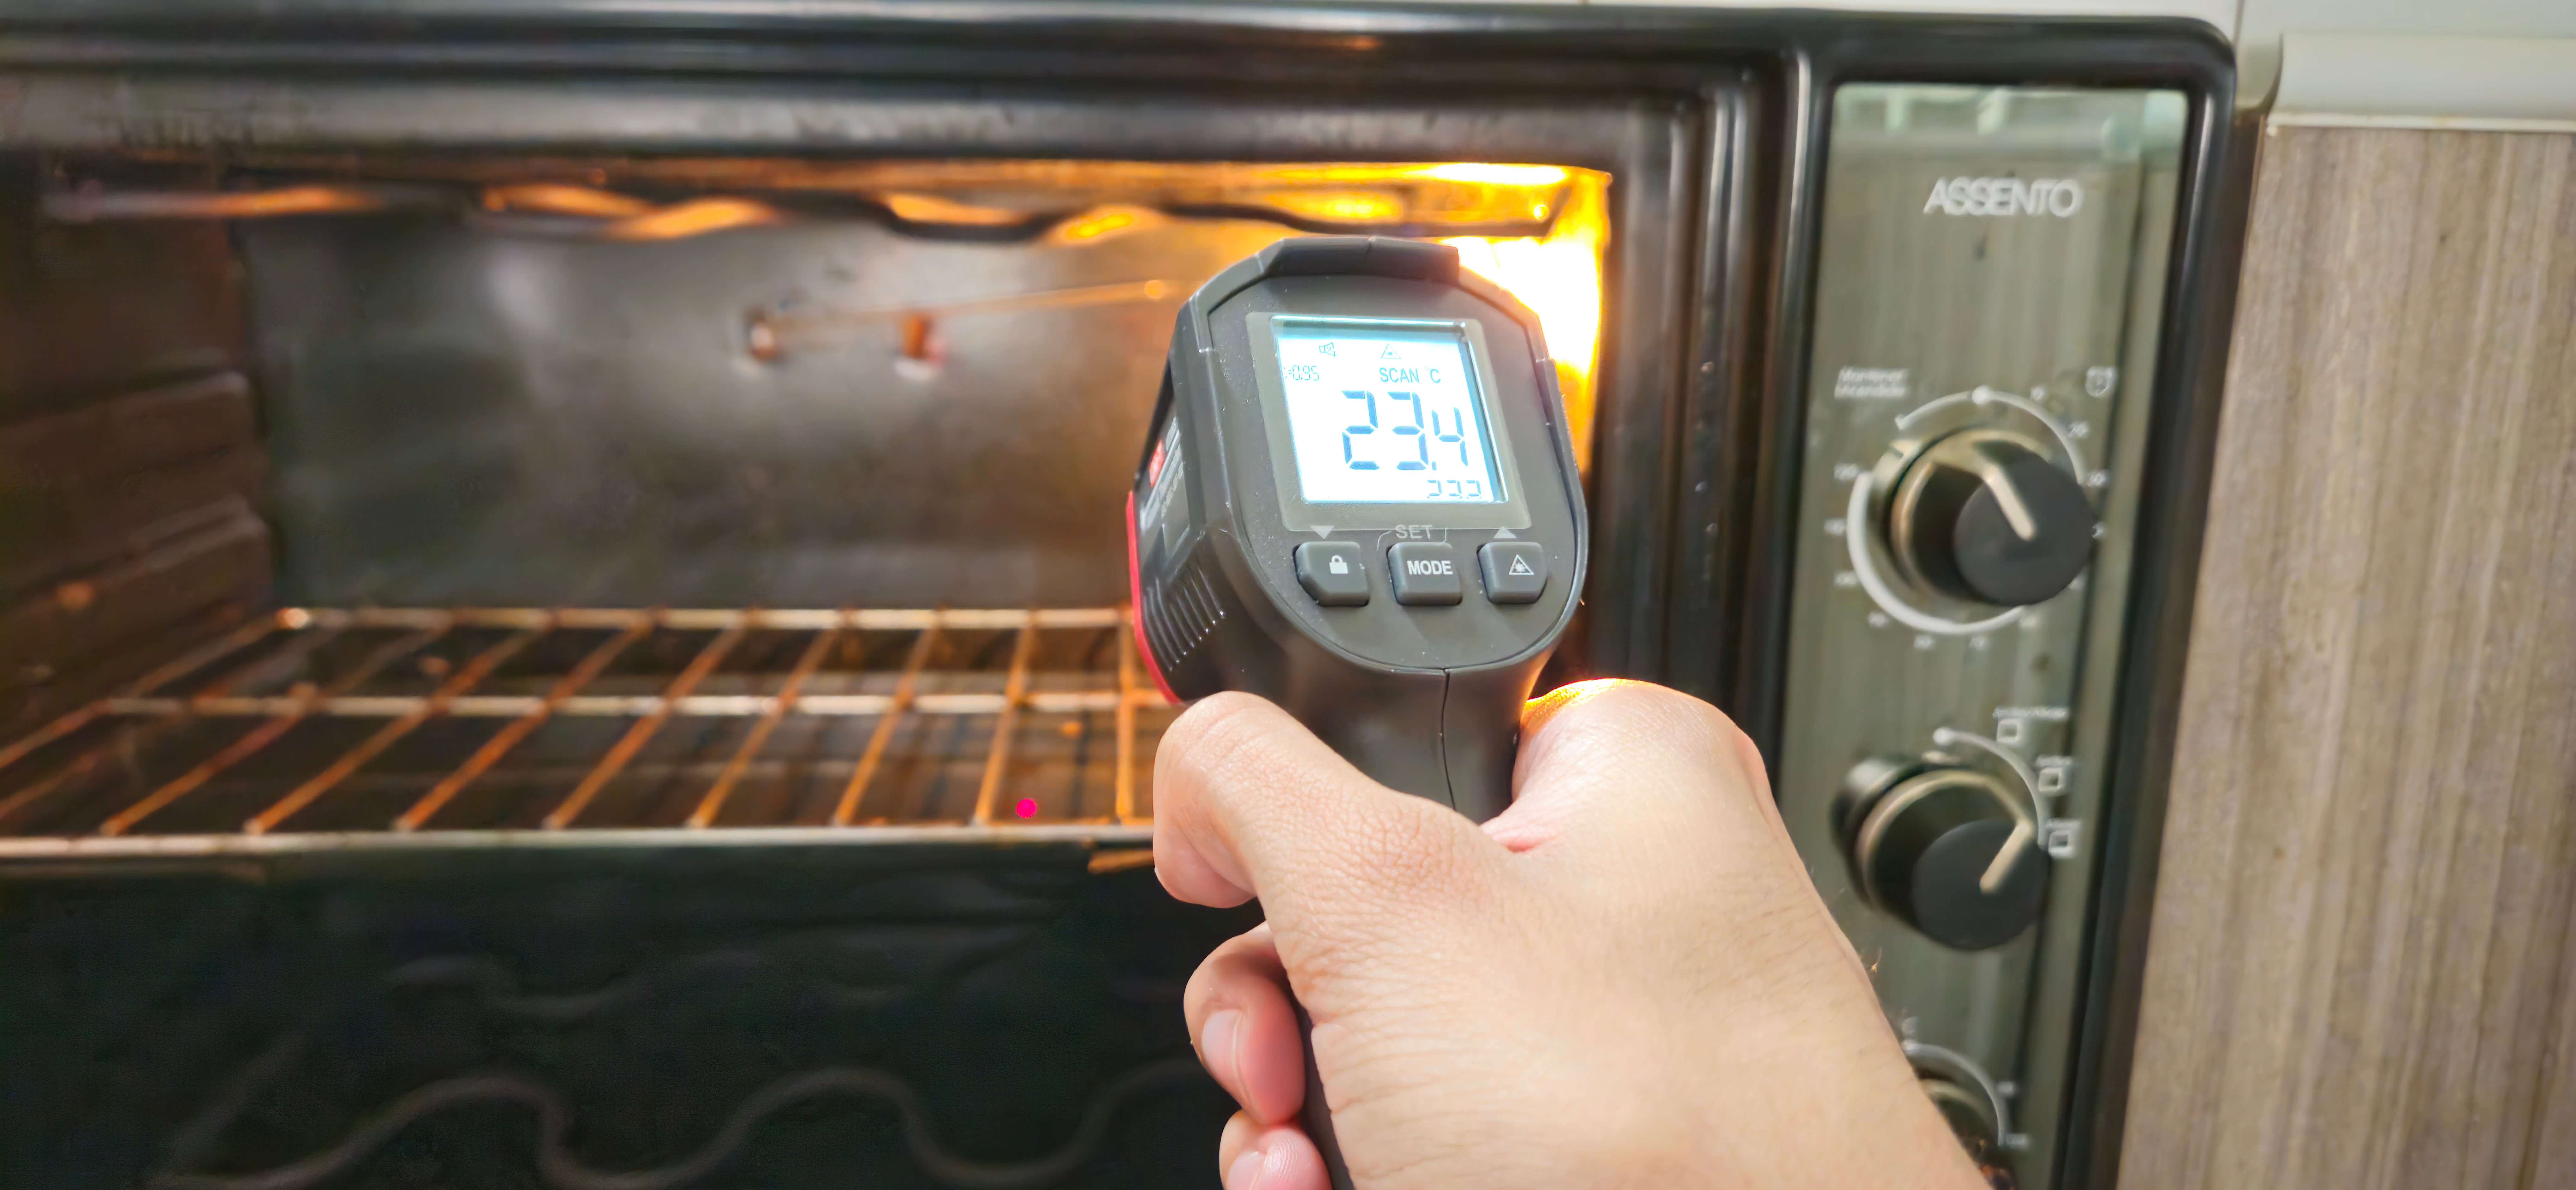
\includegraphics[width=0.9\linewidth]{../Images/oven.jpg}
\end{center}
\caption{Montaje experimental.}
\label{fig:oven}
\end{figure}

